\begin{center}
{\WorkType}
\\
Тема: {\Topic}
\\
Цель: В ходе лабораторной работы необходимо научится рарабатывать с пакетным менеджером С++. 
\end{center}
Требуемое ПО:
\begin{enumerate}	
\item Visual Studio 15.6.3 и выше с установленным пакетом для разработки С++.\
\item CMake 3.11 - https://cmake.org/download
\item git - https://git-scm.com/
\item cppan - https://cppan.org/client/
\item при установке git, cmake выбрать пункт - Добавить в PATH.
\item cppan.exe скопировать в C:\ Program Files\ CMake\ bin
\end{enumerate}
Порядок выполнения:

\begin{enumerate}	
\item Запустить VS
\item Создать проект С++ -> CMake. При создание проекта снять флажок “Создать папку для проекта”.
\item Выполнить сборку созданного проекта	\item Открыть главный CMakeLists.txt (в самой верхней папке)
\item До строки add\_executable добавить\
	find\_package(CPPAN REQUIRED)\
	cppan\_add\_package(\
	pvt.cppan.demo.intel.opencv.highgui-3\
	)\
	cppan\_execute()\
\item После строки add\_executable добавить\
target\_link\_libraries(ПервыйАргументИзAddExecutable\ pvt.cppan.demo.intel.opencv.highgui\
	)\	
\end{enumerate}
\begin{center}
Программа:
\end{center}
\begingroup
\fontsize{12pt}{12pt}\selectfont
\begin{verbatim}
Код программы CMakeLists.txt:

# CMakeList.txt: проект CMake для CMakeProject1; включите исходный код и определения
# укажите здесь логику для конкретного проекта.

cmake_minimum_required (VERSION 3.8)
# Добавьте источник для исполняемого файла этого проекта.
find_package(CPPAN REQUIRED)
cppan_add_package(
pvt.cppan.demo.intel.opencv.highgui-3
)
cppan_execute()

add_executable (CMakeProject1 "CMakeProject1.cpp" "CMakeProject1.h")
target_link_libraries(CMakeProject1 pvt.cppan.demo.intel.opencv.highgui)

# TODO: Добавьте тесты и целевые объекты, если это необходимо.

Код программы CMakeProject1

// CMakeProject1.cpp: определяет точку входа для приложения.

#include <opencv2/highgui.hpp>
#include "CMakeProject1.h"

using namespace std;

int main()
{
auto i = cv::imread("D:\\КОПИЯ ФЛЭШКИ\\4 СЕМЕСТР\\
 средства разработки программного  обеспечения Пугин Е.В\\L55\\fot\\f.jpg");
i = 255 - i; // инверсия изображения\\
cv::imwrite("D:\\КОПИЯ ФЛЭШКИ\\4 СЕМЕСТР\\
Инструментальные средства разработки программного\\
 обеспечения Пугин Е.В\\L55\\fot\\fo.bmp", i);

cout << "Hello CMake." << endl;\\
return 0;
}
\end{verbatim}
\endgroup
\begin{center}
Результат работы программы:
\end{center}
\begin{figure}[h!]
	\centering
	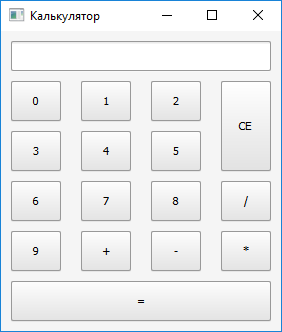
\includegraphics[scale=0.2]{s1}
	\label{fig:s1}
\end{figure}
Изображен результат работы программы.

Вывод: В ходе лаборпторной работы я научился работать с пакетным менеджером С++.



